
\section{\textit{Ray Tracing} } \label{raytracer}


Este capítulo apresenta o desenvolvimento e implementação de um simples \textit{ray tracer} usando métodos estocásticos de colisão de raios na linguagem de programação Odin com a biblioteca RayLib \footnote{\url{https://www.raylib.com/}}, usada na renderização de imagens em uma janela. Isso foi feito para começar a entender melhor as BRDFs e a equação de renderização (\autoref{eq-rendering-equation}).


O \textit{ray tracer}, que foi construído baseado no livro ``Ray Tracing in One Weekend'' \footnote{\url{https://raytracing.github.io/books/RayTracingInOneWeekend.html}}, opera inteiramente na unidade de processamento central (CPU). Sua funcionalidade principal envolve a modelagem de raios e a reflexão da cena para os \textit{pixels} da imagem. A cena consiste exclusivamente em esferas, empregando cálculos de colisão padrão entre um raio e uma esfera.


\subsection{Implementação de Materiais}


O \textit{ray tracer} inclui vários materiais que ditam o comportamento dos raios ao interagir com superfícies, os quais não são garantidos de serem fisicamente realistas em relação as propriedades de reflexão discutidas na \autoref{brdf}. Cada material é implementado como uma estrutura contendo um ponteiro de função de dispersão responsável por calcular a atenuação e o raio disperso após a interação com uma superfície. Como demonstrado no \autoref{odin-materiais}, os seguintes materiais foram implementados:


\begin{itemize}
\item \textbf{Material Difuso}: representa um material básico com refletância lambertiana.
\item \textbf{Material Lambertiano}: uma variante do material difuso com albedo personalizável.
\item \textbf{Material Metálico}: modela uma superfície metálica com reflexão especular, permitindo controle sobre a difusão.
\item \textbf{Material Dielétrico}: simula materiais transparentes com indices de refração e reflexão.
\end{itemize}


\begin{codigo}
\caption{\small Materiais.}
\label{odin-materiais}
\begin{verbatim}


Material :: struct {
    scatter: #type
        proc(self: ^Material, ray: Ray, hit: Hit)
            -> (attenuation: Color, scattered: Ray, ok: bool),
}


Shit_Diffuse_Material  :: struct {
    using _ : Material,
    albedo: Color,
}


Lambertian_Material :: struct {
    using _ : Material,
    albedo: Color,
}


Metal_Material :: struct {
    using _ : Material,
    albedo: Color,
    fuzz: f32,
}


Dielectric_Material :: struct {
    using _ : Material,
    ir: f32, // índice de refração
};
\end{verbatim}
\end{codigo}




\subsection{Mecanismo de Reflexão de Raios}


O mecanismo central do \textit{ray tracer} envolve traçar raios pela cena para determinar suas interações com superfícies e calcular os valores de cor resultantes, o resultado pode ser encontrado na \autoref{imagem-raytrace}. Esse processo foi implementado considerando os seguintes passos:


\begin{enumerate}
\item \textbf{Geração de Raios}: raios são gerados a partir do ponto de vista da câmera e projetados na cena.
\item \textbf{Detecção de Colisão}: cada raio é testado quanto à interseção com objetos na cena.
\item \textbf{Interação de Material}: após a colisão, os raios interagem com o material da superfície, determinando atenuação e raios dispersos com base nas propriedades do material.
\item \textbf{Traçado Recursivo}: se um raio se dispersa, o processo se repete, traçando o caminho do raio disperso até que uma profundidade máxima de recursão seja atingida ou o raio escape da cena.
\item \textbf{Acúmulo de Cor}: os valores de cor são acumulados ao longo do caminho do raio, essa acumulação simula a irradiância de um certo ponto da superfície.


\end{enumerate}


\begin{landscape}
\begin{figure}[H]
        \caption{\label{imagem-raytrace} \small Imagem gerada por ray tracing conforme a implementação em Odin.}
        \begin{center}
            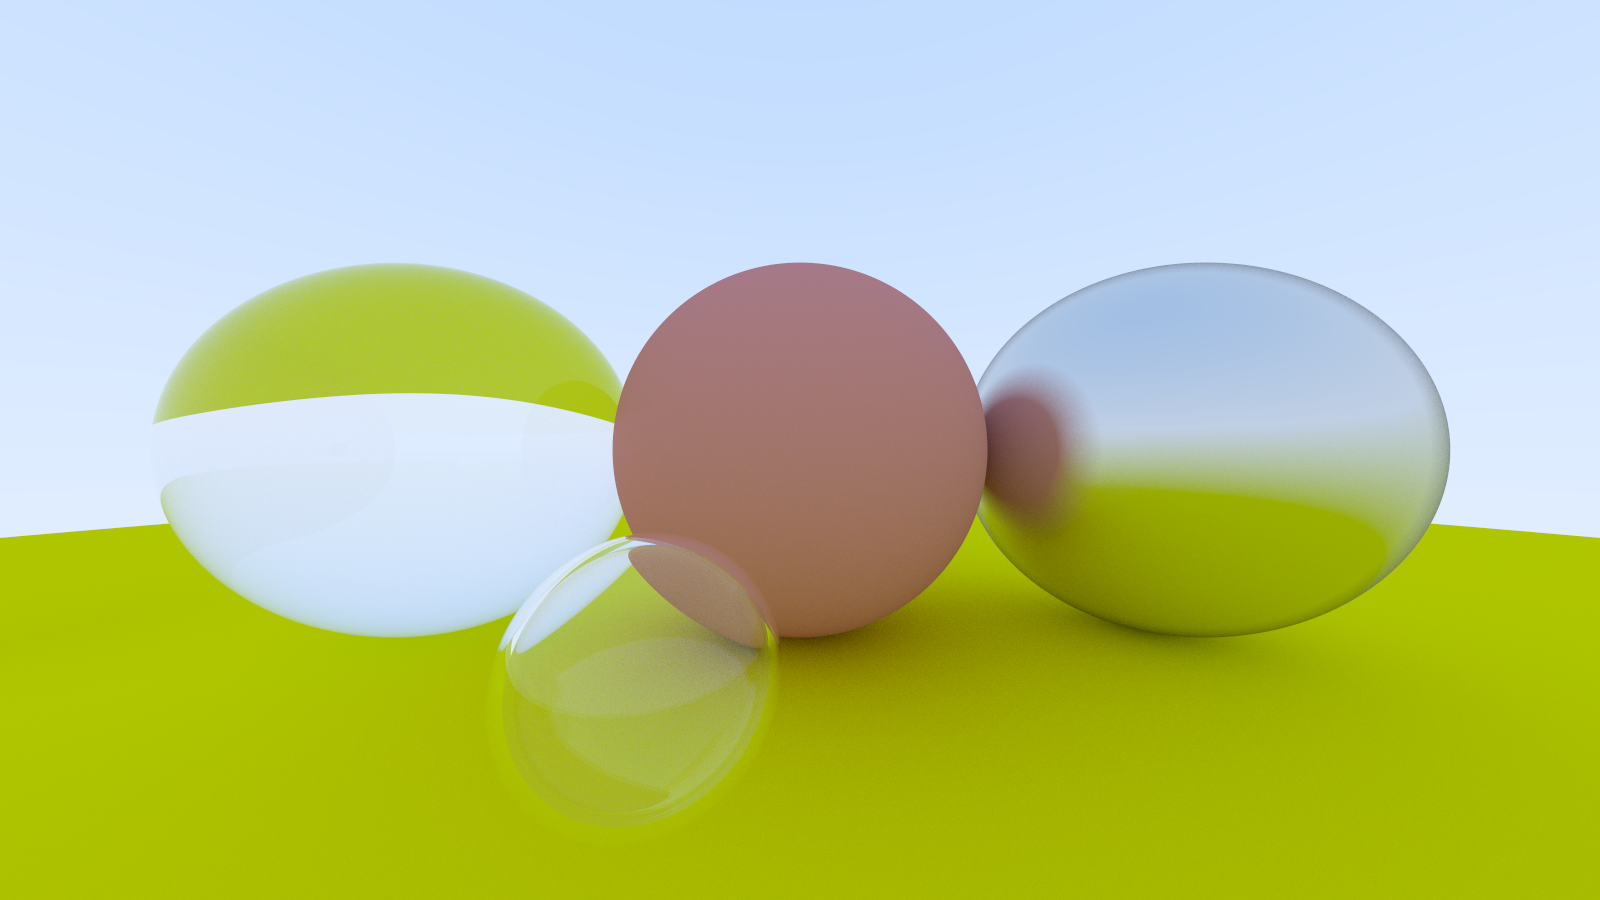
\includegraphics[scale=0.50]{./Imagens/ray_tracer.png}
        \end{center}
\end{figure}
\end{landscape}
